\section{Discussion}
\label{chap:Discussion}

\subsection{WebVectors}
\label{chap:WebVectors}

\quad The first task in this project was to play around with the \textit{WebVectors} web service 
\footnote{
\href{http://vectors.nlpl.eu/explore/embeddings/en/} {http://vectors.nlpl.eu/explore/embeddings/en/}
}. 
This web-app takes in a word and outputs a graph with 11 nodes, representing the 10 most similar words to the main input node. Edges are drawn between each of the nodes that are also very similar. The tool attempts to visualize the hyper-dimensional embedding space generated by LGT at UiO 
\footnote{\href{http://vectors.nlpl.eu/explore/embeddings/en/models/\#MOD_enwiki_upos_skipgram_300_3_2019}{http://vectors.nlpl.eu/explore/embeddings/en/models/}}
through similarities. 

\begin{figure}[H]
\centering
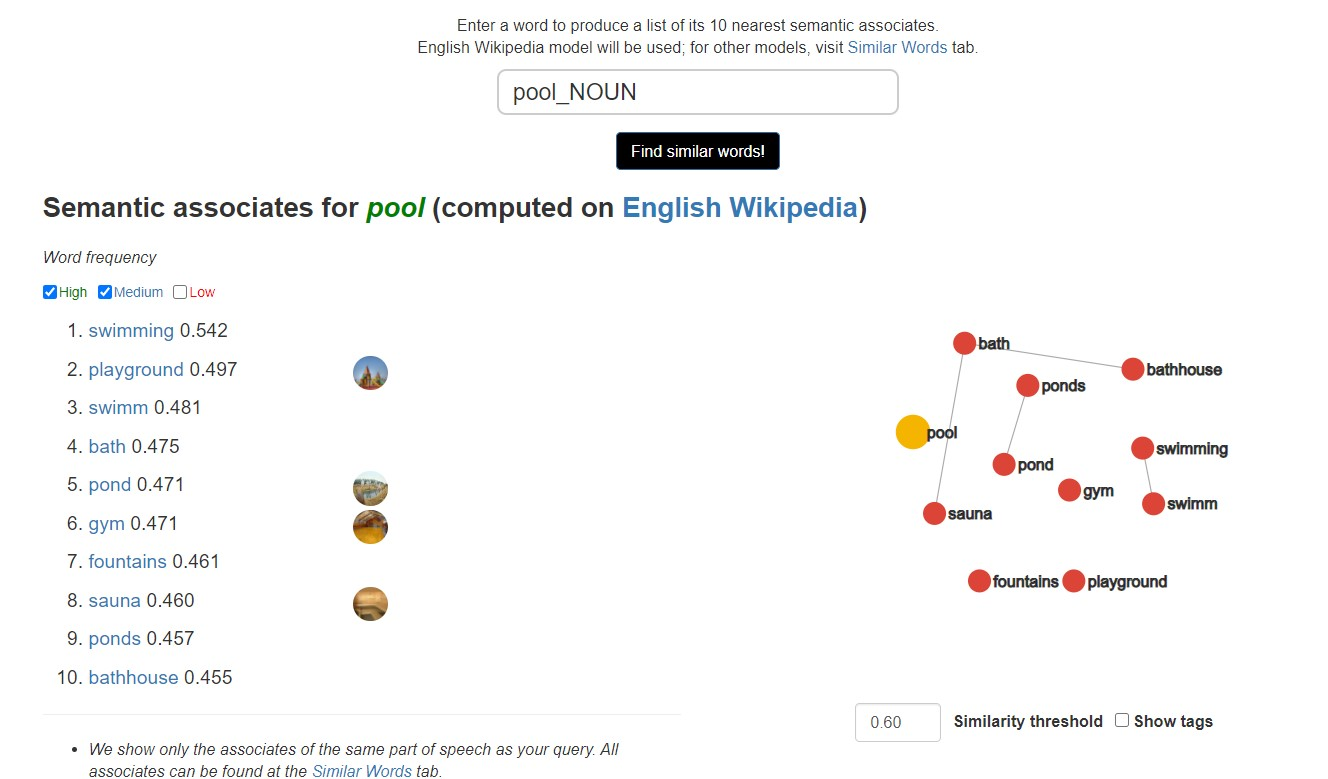
\includegraphics[width=0.75\linewidth]{pictures/pool.jpg}
\caption{WebVectors}
\end{figure}

\subsection{Working with pre-trained models locally}
\label{Chap:Working with pre-trained models locally}
\quad The next step was to load and play with the embeddings locally. This meant, reading them from the shared directory \texttt{/cluster/shared/nlpl/data/vectors/latest} on our saga login nodes. More specifically, we were to use the embedding models found at \texttt{200.zip} and \texttt{29.zip} to generate similarity tables for each word in the sentence:

\begin{quote}
    \textit{Almost all current dependency parsers classify based on millions of sparse indicator features.} \footnote{\href{https://www.aclweb.org/anthology/D14-1082.pdf}{Chen and Manning, 2014}}
\end{quote}

The provided file \texttt{play\_with\_gensim.py} gave a skeleton of how these embedding should be loaded and how the results should be presented. 
Script \texttt{\href{https://github.uio.no/fabior/IN5550/blob/master/Oblig2/ex4.py}{ex4.py}} shows our implementation of a solution for this task. 

When running this file, the user will be asked for the directory path where each of the models \texttt{200.zip} and \texttt{29.zip} lies. If the paths are correct, the output of the script can be found in \texttt{\href{https://github.uio.no/fabior/IN5550/blob/master/Oblig2/outptus/ex4/}{outputs/ex4/}}. 

The ids \texttt{200} and \texttt{29} refer to the embedding models trained on the English Wikipedia corpus and the Gigaword corpus 
\footnote{\href{http://vectors.nlpl.eu/repository/}{http://vectors.nlpl.eu/repository/}},
respectively. They both span over 300 dimensions and have respective vocabulary sizes of about 250,000 and 300,000. 

One notable difference between the two embedders is the apparent, expected case-folding of \texttt{29}, that is not present in embedder \texttt{200}. This prevents the same word from appearing in the similarity table for a specific input word, just with a capitalized first letter. This could be viewed as helpful for returning more relevant results, naturally eliminating cluttering repeats, although it would require a slightly different preprocessing technique than what was asked for here. Consequently, this tells us that the Gigaword embedding model should have more unique words and generate results for a larger span of input vocabularies. 

However, from the words tested in this example, embedder \texttt{29} actually has \textit{fewer} matches of inputs to words in its vocabulary than embedder \texttt{200}. This hints at a difference in the domain the corpora focus on.  While Gigaword has more unique words in the vocab than the Wikipedia corpus, the latter seems like a better fit for the particular domain of scientific articles. 

Further, when discussing domain adaptability, neither model was able to produce results for highly technical words like \texttt{parser}, with means both should be fine-tuned if they are to be used on this type of input data.  


%  Eivind is taking this part
\subsection{Document classification with word embeddings}
\label{chap:Document classification with word embeddings}
\quad Moving on, it came time to build a model using these embeddings as inputs. A precise formulation of the task at hand can be as follows:

\begin{quote}
    Given a list of words in a document, \textbf{predict the sentiment} of the document. 
\end{quote} 

The documents are classified as either positive or negative, which makes this a binary classification task. As it is the binary classification, we expect much higher accuracy than the last assignment (multi-class classification) as there are only two possible outputs. We reused the MLP model and used the best parameters from the last assignment as the baseline for this task. The model was modified slightly to utilize word embeddings, but the architecture remains mostly the same. 

The provided code in \texttt{play\_with\_gensim.py} was refactored to the functions \texttt{load\_embedding} and \texttt{load\_embedded\_model} in \href{https://github.uio.no/fabior/IN5550/blob/master/Oblig2/packages/preprocessing.py}{\texttt{packages/preprocessing.py}}.
\newline

\subsubsection{Baseline model}
The values for these initial parameters were chosen from the best performing model for last assignment to use as a baseline.
\begin{table}[H]
    \centering
    \begin{tabular}{ |c|c|c|c|c|c| }
        \hline
        \multicolumn{6}{|c|}{\textbf{Hyper-parameters}} \\
        \hline
        \textbf{Hidden Layers} & \textbf{Units} & \textbf{Epoch} & \textbf{Mini-batch} & \textbf{Dropout} & \texttt{Bias} \\
        \hline
        1 & 25 & 10 & 32 & 0.2 & 0.1 \\
        \hline
         \textbf{Learning Rate} & \textbf{Momentum} & \textbf{Loss-Function} & \textbf{HL-Act. Funct.} & \textbf{Out-Act. Funct.} &\\
        \hline
        0.01 & 0.9 & Cross-Entropy & tanh & relu & \\
        \hline
    \end{tabular}
    \caption{Last assignment's best performing model.}
    \label{table:baseline_params}
\end{table}

\subsubsection{Tuning}
\quad In the first assignment we made studies to determine the optimal hyperparameters for our classifier. These studies were:
\begin{itemize}
    \item \texttt{Activation function for hidden layer} $\times$ \texttt{Activation function for output layer}\newline
    $\in["sigmoid", "tanh", "relu", "softmax"]$
    \item \texttt{Number of epochs} $\times$ \texttt{Batch size}\newline
    $\in[5, 10, 15, 20, 30, 40, 50]$
    $\times$
    $\in[32, 35, 40, 45, 50, 500]$
    \item \texttt{Number of hidden layers} $\times$ \texttt{Number of units per layer}\newline
    $\in[1, 2, 3, 4]$
    $\times$
    $\in[5, 10, 25, 50, 100, 250, 500, 1000, 2000]$
    \item \texttt{Learning rate} $\times$ \texttt{Momentum}\newline
    $\in[0.5, 0.1, 0.05, 0.01, 0.005, 0.001]$
    $\times$
    $\in[0.9, 0.7, 0.5, 0.3, 0.1, 0]$
\end{itemize}

We opted to make the tuning more automized this time, with a dynamic evaluation function \href{https://github.uio.no/fabior/IN5550/blob/master/Oblig2/ex5.py}{\texttt{ex5.py}}. This function swaps out the default parameter with the one yielding the best result from the studies in \href{https://github.uio.no/fabior/IN5550/blob/master/Oblig2/packages/studies.py}{\texttt{packages/studies.py}}. This module consists of multiple different \texttt{Study} classes for each of the different parameter pairs this group decided to test. The encapsulation of the classes helped maintain efficient memory usage and made for straightforward and understandable tuning. 

A \href{https://github.uio.no/fabior/IN5550/blob/master/Oblig2/packages/ex5.py}{\texttt{packages/ex5.py}} script executed the studies for each of the tuning steps. It was this file that generated the results presented below. These results are stored in the   \href{https://github.uio.no/fabior/IN5550/blob/master/Oblig2/ex5}{\texttt{output/ex5}} directory. For this assignment, the most important metric we looked at was accuracy.

Before running the studies from the last assignment, we first had to find a vocabulary suited for our task. Thus additional tuning was required, as there were many pre-trained vocabularies to choose from, and we had observed spikes in accuracy when choosing the word embedding model arbitrarily. We created two more studies:
\begin{itemize}
    \item Testing pretrained vocabularies against different loss functions.
    \item Testing different word embedding types against the pretrained vocabularies.
\end{itemize}
\quad This was mainly to find an optimal vocabulary to use, as well as asserting that cross entropy was a good loss function to utilize.\newline

The combination that yielded the best result was vocabulary 40, a Word2Vec Continous Skipgram without POS tagging, and cross-entropy. Thus we continued with vocabulary 40 and cross-entropy. 

Once we had found our preferred word embedding model, we decided on the type of embedding we were going to use.

\quad As we can see in \href{fig:emb_type}{the heatmap}, the mean was by the far superior embedding type, and the model was finally producing actual results. After finding the appropriate vocabulary and embedding type, we could tune the model in the same manner as in the previous assignment.

\begin{table}[H]
    \centering
    \begin{tabular}{c|c|c|c}
        \textbf{Study} & \textbf{Param. 1} & \textbf{Param. 2} & \textbf{Heatmap}\\
        \hline
        \texttt{VocabLossFunct} &  \texttt{Loss function: cross-entropy}  &  \texttt{Vocabulary: 40} & Apendix \ref{fig:vocabloss_ex5} \\
        \texttt{EmbedTypeNewVocab} &  \texttt{Embedding type: mean}  &  \texttt{} & Apendix \ref{fig:embtypestudy_ex5} \\
        \texttt{ActFunct} &  \texttt{Hidden: tanh}  &  \texttt{Output: relu} & Apendix \ref{fig:actfunct_ex5} \\
        \texttt{EpochsBatches} &  \texttt{Epochs:30}  &  \texttt{Batch size:32} & Apendix \ref{fig:epochbatch_ex5} \\
        \texttt{HLU} &  \texttt{Hidden layers:2}  &  \texttt{Units:5} & Apendix \ref{fig:hlu_ex5} \\
        \texttt{LrMmt} &  \texttt{Learning rate: 0.01}  &  \texttt{Momentum: 0.9} & Apendix \ref{fig:lrmmt_ex5}\\
    \end{tabular}
    \caption{Results from studies of exercise 5}
    \label{tab:ex5_studies}
\end{table}

  

\subsubsection{Optimal parameters for MLP model}
The best parameters for the MLP model can be seen in \href{table:optimal_params}{the table below} which received an accuracy score of 0.694.
\begin{table}[H]
    \centering
    \begin{tabular}{ |c|c|c|c|c| }
        \hline
        \multicolumn{5}{|c|}{\textbf{Hyper-parameters for MLP model}} \\
        \hline
        \textbf{Hidden Layers} & \textbf{Units} & \textbf{Epoch} & \textbf{Mini-batch} & \textbf{Dropout} \\
        \hline
        1 & 25 & 10 & 32 & 0.2 \\
        \hline
         \textbf{Learning Rate} & \textbf{Momentum} & \textbf{Loss-Function} & \textbf{HL-Act. Funct.} &\\
        \hline
        0.01 & 0.9 & Cross-Entropy & tanh & \\
        \hline
         \textbf{Embedding type} & \texttt{Vocabulary} & \textbf{Bias} & \textbf{Out-Act. Funct.} &\\
         \hline
         mean & 40 & 0.1 & relu &\\
        \hline
    \end{tabular}
    \caption{The best hyperparameters found for the MLP model.}
    \label{table:optimal_params}
\end{table}

These were used as the default values for the upcoming steps in our analysis.

%  Per will start part 6
\subsection{Document classification using recurrent neural networks}
\label{chap:Document classification using recurrent neural networks}

\quad The next part of this project was to implement a RNN as a classifier. We were to continue the task from part \ref{chap:Document classification with word embeddings}, where the goal was to classify the sentiment polarity of an input sentence. We chose to only focus on fine-tuning the RNN and feeding it forward to a single linear output layer for simplicity. This way, we can directly compare the performance of recurrent networks with simple, feed-forward networks, as implemented above, getting a precise measurement of the increase of performance these architectures bring. 

Recurrent neural networks work well on sentiment analysis because they maintain the inherent, sequential information of input sentences. The order in which words appear in a sentence can change the sentence's overall polarity. For example, take the two sentences:

\begin{quote}
    In contrast to the \textbf{poor} title, the movie was overall \textbf{interesting}.
\end{quote}
\begin{quote}
    In contrast to the \textbf{interesting} title, the movie was overall \textbf{poor}. 
\end{quote}

The two sentences carry opposite polarities, yet a bag-of-words model would classify them exactly the same. Through element-wise updating of states, RNN's consider each word concerning all of the preceding words. This allows the model to capture some of the sentence's structural information, making it more likely to predict the correct sentiment of the sentence. 

Specific RNN flavors (LSTM and GRU) incorporate \textit{gated architectures}. Simply put, these learn to separate between the input features that the model needs to focus on from those that are best left untouched. The gates then filter and feed-forward only the features that need tuning, sending the others directly to the output, thus preventing ambiguous computation and over-fitting.

To get a feel of both gated and non-gated RNN's, we were asked to experiment with PyTorch's three RNN types
\footnote{
\href{https://pytorch.org/docs/1.7.1/nn.html\#recurrent-layers}{Recurrent Layers in PyTorch (1.7.1)}
}, and report the results on the variations of performance. 

\subsubsection{Building the model}
\label{chap:builingrnn}

\quad The underlying structure of the \texttt{MLPModel} was reused, but with some slight alterations. The \texttt{self.model} attribute was set to an instance of a PyTorch RNN, dependent upon the hyperparameter \texttt{rnn\_type:str="rnn"} of the \texttt{RNNModel} class. The three possible alternatives here were: \texttt{"rnn"}, \texttt{"lstm}, or \texttt{"gru"}.

Another part of the model that changed from that used in part \ref{chap:Document classification with word embeddings} was the output layer. For the RNN architectures, a \texttt{self.\_linear} attribute was used, instead of the \texttt{self.out} from above. This allowed for the model to predict the two classes independently of each other, which translates to higher model flexibility. Additionally, limiting the complexity of the output layer allowed for more direct observations on the performance of RNNs. 

The linear layer's input size depended on the size of the output the RNN layer would be serving. In particular, if the RNN layer was given the parameter \texttt{bidirectional=True}, the output size would double, moreover the linear layer's input size would need to be doubled. Bidirectional recurrent network outputs are two times larger than regular recurrent networks because they return updated state values from reading the input both forward and backward. 

It was still preferable to convert the input text to word embeddings since we saw an increase in performance from the bag of words model in classification with word embeddings. This meant that again, the model needed a \texttt{torch.nn.Embedding} attribute to convert input data into embedding representations. This was kept open as a tunable parameter since the optimal embedding vocabulary for a simple feed-forward network is not necessarily the optimal vocabulary for an RNN. The optimal embedder is something that needs to be found for each architecture. 

One last key element of our implementation of
\texttt{\href{https://github.uio.no/fabior/IN5550/blob/master/Oblig2/packages/ann_models.py}{RNNModel}}
was the incorporation of a learning rate scheduler. While there are many different solutions to adaptive learning rates for neural architectures, we chose to utilize the \texttt{torch.optim.lr\_scheduler.ReduceLROnPlateau} variant. This tool's idea is to adjust the learning rate every time learning seems to stagnate, making sure the model is always learning as much as possible without overfitting. We felt this was necessary because we noticed the loss would often decrease for a few epochs and then jump back up. This told us the optimizer was overstepping, which meant the learning rate was too high. The scheduler fixed this problem. A vital drawback here is that the scheduler only works in one direction and cannot self-correct if an adjustment occurs prematurely.

\subsubsection{Tuning studies}
\quad Similar to those developed for the \texttt{MLPModel}, a set of studies were created to test different variations of architectures of recurrent neural networks found in \texttt{\href{https://github.uio.no/fabior/IN5550/blob/master/Oblig2/packages/rnn\_studies.py}{rnn\_studies.py}}. While some of the studies were able to be reused as-is, quite a few new studies needed to be written. The new study implementations here included:

\begin{itemize}
    \item \texttt{RnnTypeBiDirectional}
    \item \texttt{VocabRnnType}
    \item \texttt{PoolTypeRnnType}
    \item \texttt{BestEpochRnnType}
    \item \texttt{FactorPatience}
\end{itemize}

We tested one more parameter but did not develop a study for the freezing/unfreezing of the model's embeddings. Analysis of this parameter was done using the bidirectional study, manually changing the value for this parameter. The freezing of embeddings means that they will \textit{not} be updated according to how much the model learned for each epoch. This means they will not be fine-tuned for the particular vocabulary being worked on, thus simplifying the model's complexity. It can often be beneficial to fine-tune a model's embeddings if the task at hand includes many unique words particular to the task's respective domain, which seemed to not happen in this assignment. Word embedding models train to span over as general of a vocabulary as possible to prevent the need for future fine-tuning, as computation time should always be minimized. 

\begin{figure}[H]
    \centering
    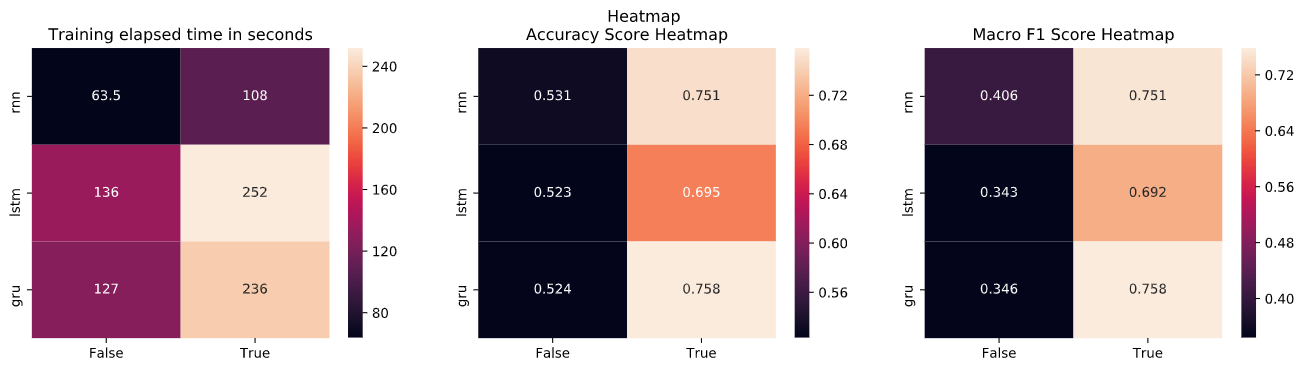
\includegraphics[width=1\linewidth]{pictures/RnnTypeBiDirectional_freeze_true_heatmap.png}
    \caption{Freeze = True}
    \label{fig:freeze_true}
\end{figure}

\begin{figure}[H]
    \centering
    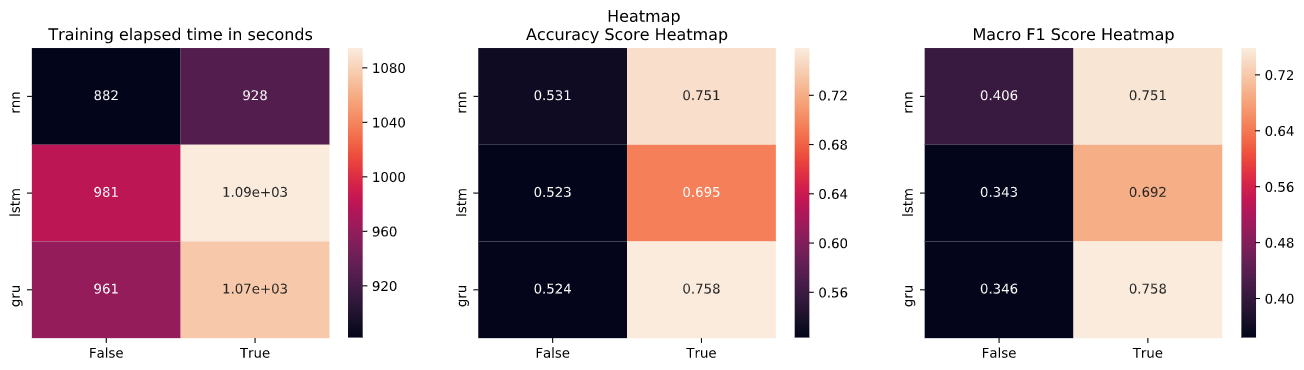
\includegraphics[width=1\linewidth]{pictures/RnnTypeBiDirectional_freeze_false_heatmap.png}
    \caption{Freeze = False}
    \label{fig:freeze_false}
\end{figure}

As can be seen when comparing figures \ref{fig:freeze_true} and \ref{fig:freeze_false}, the only major difference between frozen and non-frozen embeddings was the computation time. Our model could not truly fine-tune the embeddings (LGT did too good a job when training them). For the rest of the experiments, we kept \texttt{freeze=True} to lower computation times. 

\paragraph{RNN type versus Bidirectional}
Some of the results from the first study have already been shown. The \texttt{True}/\texttt{False} axes in figures \ref{fig:freeze_true} and \ref{fig:freeze_false} represent the \texttt{bidirectional} parameter. As can be seen, only reliable results were found when bidirectional was activated. This tells us that a lot can be learned from these particular data about the sentence structure by feeding it to the model both forward and backward. It is important to note here that this study only intended on finding the optimal value for bidirectional. We wanted to test the different RNN types with some of the other variables as well, so no optimal RNN was derived from these analyses. 

\paragraph{Embedding vocabulary versus RNN type}
Next, we wanted to find which embedding vocabulary worked best for each of the three RNN types. We assume that these optimal vocabularies would be different from those found for the MLP model but needed empirical evidence to support this claim.

\begin{figure}[H]
    \centering
    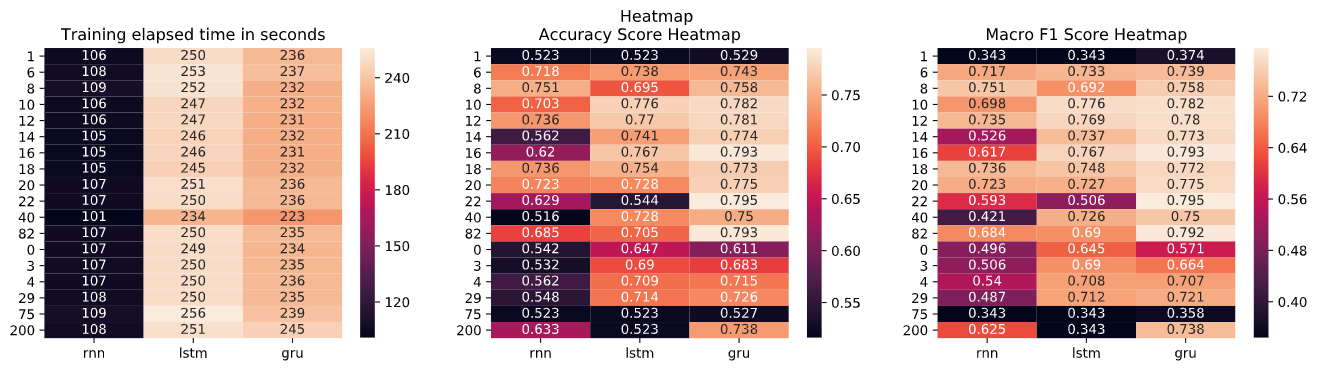
\includegraphics[width=1\linewidth]{pictures/VocabRnnType_heatmap.png}
    \caption{Embedding vocab versus RNN type}
    \label{fig:vocab_rnn}
\end{figure}

Figure \ref{fig:vocab_rnn} shows the results of this study, although the individual vocabularies are only specified by their ID. The 3 top performing vocabularies were as followed:
\begin{center}
    \begin{tabular}{c|c|c|c}
        \textbf{Rank}   & \textbf{1$^\text{st}$} & \textbf{ 2$^\text{nd}$} & \textbf{3$^\text{rd}$} \\
        \hline
        \textbf{Algorithm} & fastText Skipgram & fastText Skipgram & Global Vectors \\
        \hline
        \textbf{ID}     & 22  & 16  & 82 \\ 
        \hline
        \textbf{Corpus} & Wikipedia'17 + Gigaword 5th & Gigaword 5th  &  English Common Crawl  \\
        \hline
        \textbf{Vocab. Size} & 291392 & 292967 & 2000000  \\
        \hline
        \hline
        \textbf{Accuracy} & 79.5\% & 79.3\% & 79.3\%    \\
        \hline
        \textbf{F-Score 1} & 79.5\% & 79.3\% & 79.2\%    \\
    \end{tabular}
\end{center}

An interesting point to note here is that the top 2 embedding models were built using the fastText skipgram algorithm. The Global Vectors algorithm also achieved scores close to that of fastText, across the board, barely missing out on that top spot. Comparatively, the vocabulary size difference between these two embedding algorithms highlights the efficiency of the former. This makes sense since the latter is one of the more rudimentary embedding techniques in the field, built on count matrices of individual words and how often they co-occur together. FastText uses a more robust approach, focusing on n-grams of all shapes, not just singular words. This opens the possibility of representing higher-level concepts and abstractions than previously possible, which is intuitively quite important in language analysis since language is a higher-level abstraction of the human experience.

Another thing to note from this study is the absence of the POS vocabularies as the top performers. All of the English embedders present in the embedding repository [\ref{Bib:embeddingrepo}], including all of those which incorporated part-of-speech tags, were tested here. However, only a few of the POS tagged embedders gave results indicating that the model \textit{actually} learned something. This could have been because the POS tagging technique we used might not have been 100\% similar to that which trained those models. Regardless, the models that returned the poorest scores were excluded from the heatmaps for visibility, but their results can still be found in the \href{https://github.uio.no/fabior/IN5550/tree/master/Oblig2/outputs/}{\texttt{outputs/}} directory. 

Finally, since the difference between performances of 22 and 16 were quite small, we decided to test both of them in some of the upcoming studies to see if any variations in performance would reveal themselves in the later optimization stages.

\paragraph{Pooling strategy versus RNN types}
The next natural parameter to study was the pooling strategy applied after the RNN. Simply put, this step converted the 3-dimensional output from the RNN to a 2-dimensional (and linearly interpretable) tensor through some pooling technique. The three techniques we limited our analysis to were slicing the first layer of weights (states) from the RNN output, the last layer, and a concatenation of the two. We also looked slightly into max-pooling (finding the weights with the highest values for each node position, through all the layers of the RNN) and average pooling (average values of each node position through all the layers), but the results seemed too unreliable to include in this report. 

We needed to look at both the front slice and the back slice of the output because of bidirectional being set to true (as stated above). Technically, after the model is finished learning, the last spot that would have been updated is that at the first index of the network, since information flowed through the model twice, once from front-to-back and again back-to-front. So, intuitively, this layer provides the most condensed version of the information learned by the model.

\begin{figure}[H]
    \centering
    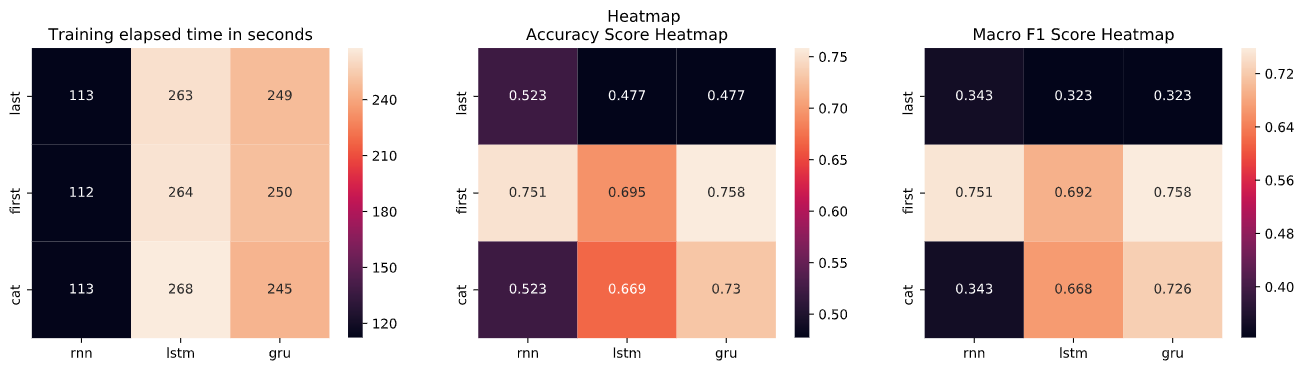
\includegraphics[width=1\linewidth]{pictures/PoolTypeRnnType_heatmap.png}
    \caption{Pooling strategy versus RNN type}
    \label{fig:pool_rnn}
\end{figure}

The evidence in the heatmaps shown in Figure \ref{fig:pool_rnn} prove the point made in the previous paragraph. The scores for the models using the \texttt{last} pooling strategy gave very poor results (basically random guessing). The technique that read only the \texttt{first} slice scored the best, with the concatenation of the two in a close second place (surprisingly enough). 

\paragraph{RNN type and best epoch}
One study that wouldn't look so pretty in a heat map was the one used to determine the actual best RNN type. Using the optimal hyperparameters found so far, this study also looked at the number of epochs it took each architecture type to reach it's highest performance. Noise could play a very large factor here, so heatmaps were disregarded and the results are therefore presented in Table \ref{tab:rnn_type}:

\begin{table}[H]
    \centering
    \begin{tabular}{c|c|c|c}
        \textbf{type}    & Elman & LSTM & GRU  \\
        \hline
        \textbf{accuracy}   & 72.5\% & 80.7\% & 80.2\% \\
        \hline
        \textbf{epochs}  & 34    & 86    & 58  \\
    \end{tabular}
    \caption{RNN type study}
    \label{tab:rnn_type}
\end{table}

This study was quite interesting, especially with the learning rate scheduler enabled because every bounce up of the loss, indicating over-fitting, resulted in the learning rate being lowed by the scheduler. With a very shallow learning rate, near 0, the model's learning ability does not change anymore, staying in the highest accuracy without over-fitting.

For all three architectures, the performance pretty much reached the converging range after around 30 epochs. However the best performances weren't actually reached until much later (two to three times as many epochs later). This insight was applied to the later studies, testing only on 30 epochs for lighter computing resources, with the intentions to train the final model on many more.

We're also confident the model wasn't over-fitting (at least not by a substantial amount) because of the scheduler. In fact, when studying the output for this study, it was observed that every time there was an increase in loss for a few steps, the model seemed to correct itself, and start learning again. 

This output was stored in \href{https://github.uio.no/fabior/IN5550/tree/master/Oblig27/outputs/ex6/slurm_PoolTypeRnnType_and_BestEpochRnnType_vocab22.out}
{outputs/ex6/slurm\_BestEpochRnnType\_vocab22.out}, and gives a nice insight in the optimal ranges for epochs for these architectures on these data.

In this study, the chosen RNN type was GRU because of its efficiency, relatively high score with fewer epochs. Indeed, the score difference between LSTM and GRU was not significant; therefore, the lower number of epochs was considered an efficiency parameter.

\paragraph{Hidden layer versus units}
The exact same hidden layers versus units study was used from previous experiments. The only maps that showed a true trend were the time maps.

\begin{figure}[H]
    \centering
    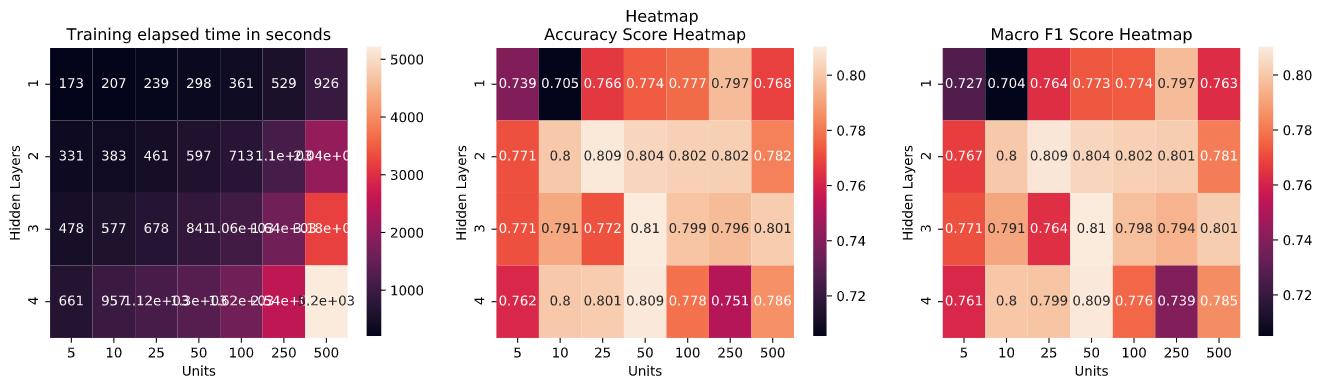
\includegraphics[width=1\linewidth]{pictures/ex6_heatmap_16_HLUnits.png}
    \caption{Hidden layers vs. Units (vocab. 16)}
    \label{fig:hlu_16_rnn}
\end{figure}

\begin{figure}[H]
    \centering
    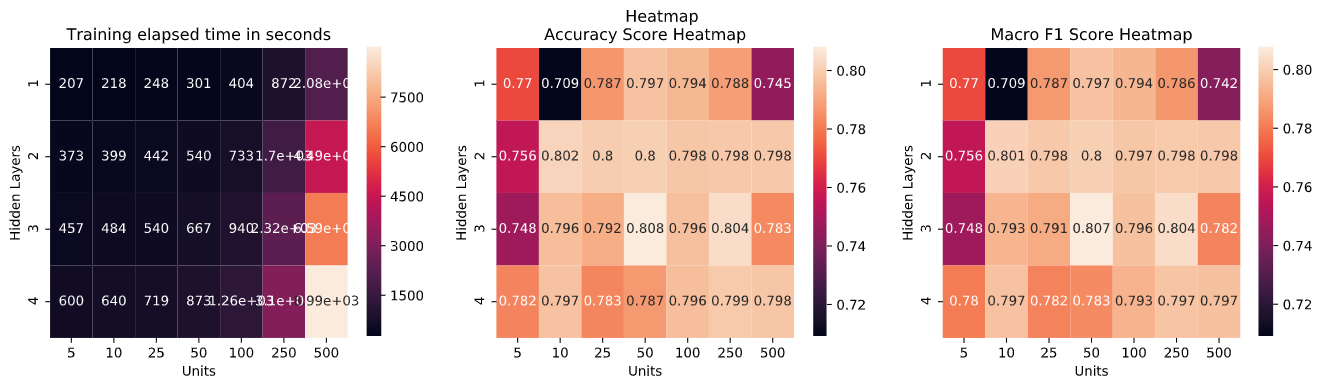
\includegraphics[width=1\linewidth]{pictures/ex6_heatmap_22_HLUnits.png}
    \caption{Hidden layers vs. Units (vocab. 22)}
    \label{fig:hlu_22_rnn}
\end{figure}

However, it is interesting to point out that both embedding 16 and 22 gave the best score with 3 hidden layers and 50 units. Figure \ref{fig:hlu_16_rnn} shows a very close second place at 2 hidden layers and only 25 units. Again, to spare excess computations, these values were deemed good enough for future experiments (with intentions of using the 3 hidden and 50 units on the final model).

\paragraph{Learning rate versus momentum}
The next study was also one that has been used previously, namely comparing learning rates against momentum. Recall the learning rate scheduler implemented here, that only \textit{reduces} the learning rate on stagnation. This tells us that larger start values for learning rate are probably better than small, since they give the scheduler more control and ability to work properly. 

Momentum is obviously chosen the test with learning rate, since the two parameters are highly correlated. Lower learning rates require higher momentum, ensuring the model learns enough each epoch to produce a noticeable change in performance. 

Again, both vocabulary 16 and 22 were tested simultaneously.

\begin{figure}[H]
    \centering
    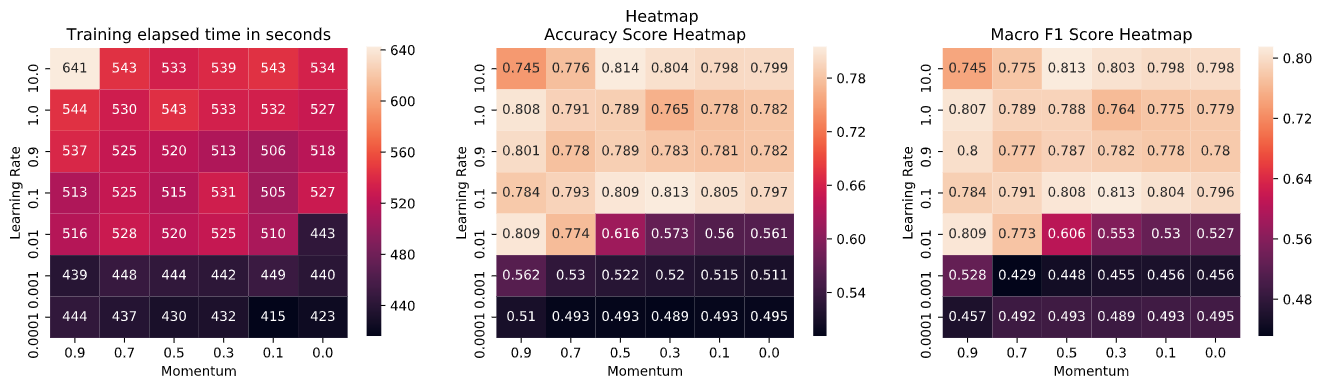
\includegraphics[width=1\linewidth]{pictures/ex6_heatmap_16_LrMmt.png}
    \caption{Learning rate vs. Momentum (vocab. 16)}
    \label{fig:lrm_16_rnn}
\end{figure}

\begin{figure}[H]
    \centering
    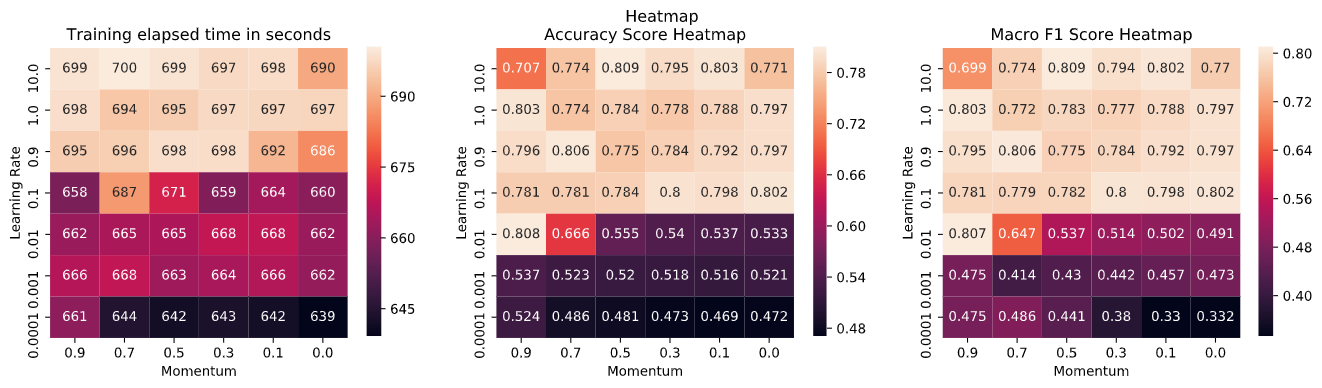
\includegraphics[width=1\linewidth]{pictures/ex6_heatmap_22_LrMmt.png}
    \caption{Learning rate vs. Momentum (vocab. 22)}
    \label{fig:lrm_22_rnn}
\end{figure}

Just to see what would happen, we tested a learning rate of 10, even though this does not quite make theoretical sense. To our surprise, this actually gave some of the better results. Most likely, this elevated performance came from the ultimate flexibility we are giving the scheduler here. The current factor being tested was 0.1, so after the scheduler's first reduction, the learning rate would be back down to "normal" values.  

We decided to shoot safe and stick to the best performing learning rate between 0 and 1, which was 0.1. This occurred with a momentum of 0.3, which is much lower than found for previous neural architectures' implementations. This is likely due to the inherent complexity of RNNs, which do not rely as much on previous performance improvement than the vanilla MLP model from above.

\paragraph{Factor versus patience}
Two completely new parameters that needed to be tuned here were \texttt{factor} and \texttt{patience} of the learning rate scheduler. 
Factor refers to how much the scheduler should reduce the learning rate when called. Patience is how many epochs are allowed after stagnation is first noticed, before calling for a reduction. 

\begin{figure}[H]
    \centering
    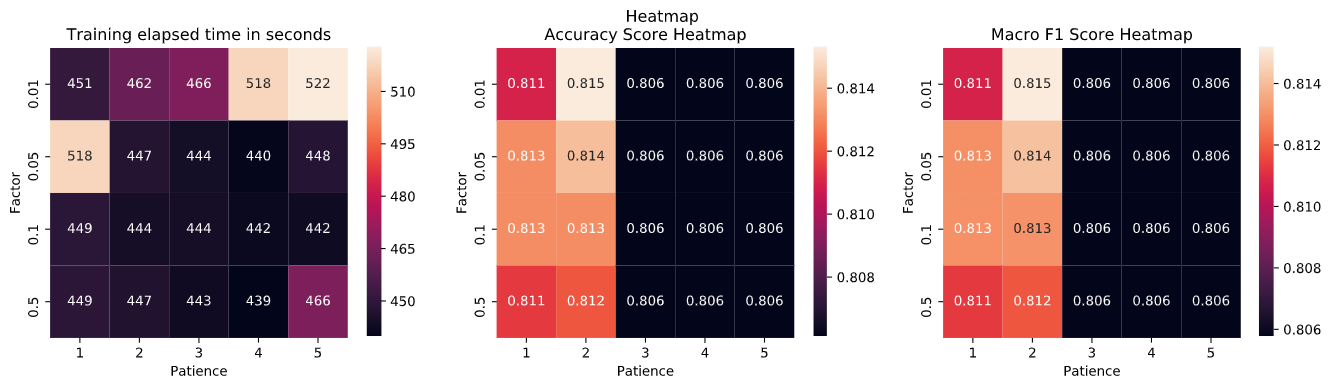
\includegraphics[width=1\linewidth]{pictures/ex6_heatmap_16_FactorPatience.png}
    \caption{Factor vs. Patience (vocab. 16)}
    \label{fig:factor_16_rnn}
\end{figure}

\begin{figure}[H]
    \centering
    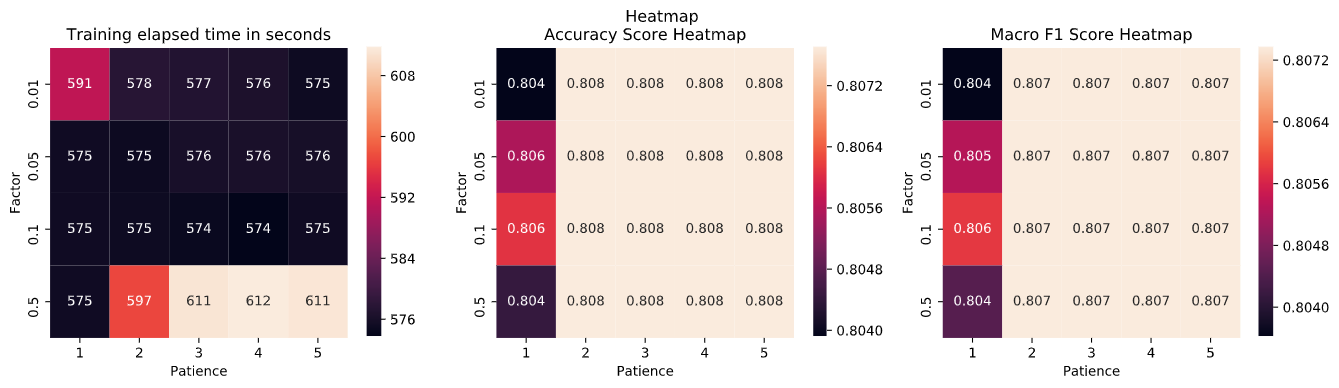
\includegraphics[width=1\linewidth]{pictures/ex6_heatmap_22_FactorPatience.png}
    \caption{Factor vs. Pateience (vocab. 22)}
    \label{fig:factor_22_rnn}
\end{figure}

Figures \ref{fig:factor_16_rnn} and \ref{fig:factor_22_rnn} show very little variation in performance when tuning of these values. However, a factor of 0.01 and patience of 2 is the top scoring configuration, when considering both embedders. 

\paragraph{Batch size versus number of epochs}
The final study run in this analysis tested different batch sizes with number of epochs (repeated to reuse previous \href{https://github.uio.no/fabior/IN5550/blob/master/Oblig2/packages/studies.py}{study}). We wanted to make sure the batch size used for these tests were defendable. 

\begin{figure}[H]
    \centering
    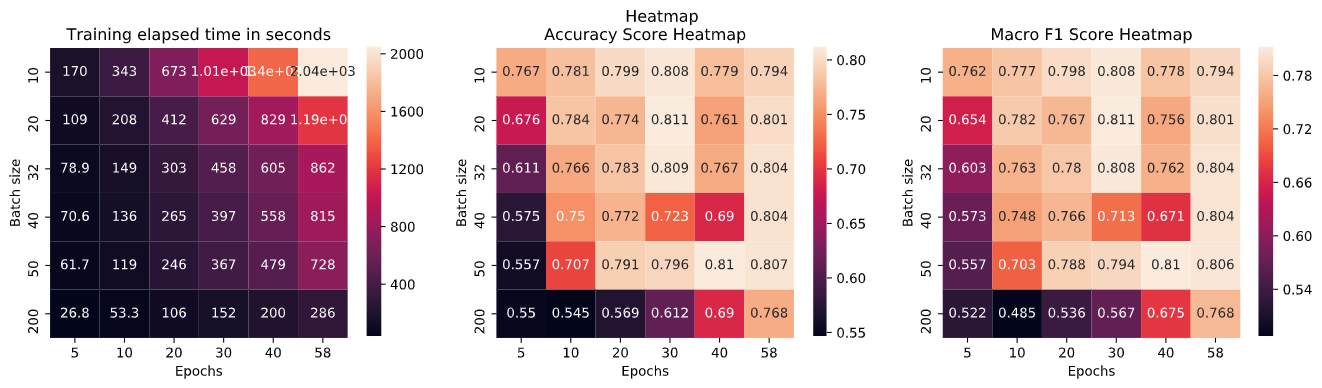
\includegraphics[width=1\linewidth]{pictures/ex6_heatmap_16_BatchEpoch.png}
    \caption{Batch size vs. Epochs (Vocab. 16)}
    \label{fig:batch_epoch_rnn}
\end{figure}
\begin{figure}[H]
    \centering
    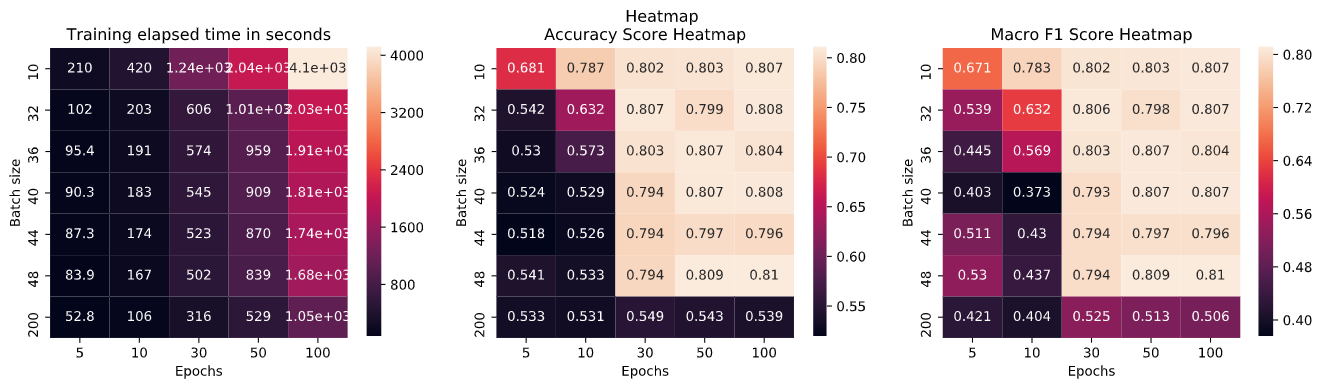
\includegraphics[width=1\linewidth]{pictures/ex6_heatmap_22_BatchEpoch.png}
    \caption{Batch size vs. Epochs (Vocab. 22)}
    \label{fig:batch_epoch_22_rnn}
\end{figure}

A key insight to note here is the \textit{poor} performance with too few epochs and too large of batch sizes. Other than that, it seemed we were already testing pretty close to the optimal parameters, with both around 30.


\subsection{Final hyperparameters}
\label{chap:Final hyperparameters}
\quad As a result of our experimenting, our setup gave the following optimal hyperparameters:

\begin{table}[H]
    \centering
    \begin{tabular}{ |c|c|c|c|c|c| }
        % \hline
        % \multicolumn{6}{|c|}{\textbf{Final model hyperparameters}} \\
        \hline
        \textbf{Vocab}  & \textbf{RNN} & \textbf{Bidirection/Freeze}  &  \textbf{Pool}  & \textbf{Batch size} &\textbf{Epoch}\\
        \hline
        22 & GRU & True / True & First & 20 & 30 \\
        \hline
         \textbf{Learning Rate} & \textbf{Momentum} & \textbf{Factor} & \textbf{Patience} & \textbf{Hidden Layers} & \textbf{Units} \\
        \hline
        0.01 & 0.9 & 0.01 & 2 & 3 & 50\\
        \hline
    \end{tabular}
    \caption{Optimized model parameters}
    \label{table:final_params}
\end{table}
